% \documentclass[twocolumn]{article}
\documentclass[]{article}
\usepackage[left=20mm, right=20mm, top=20mm, bottom=20mm]{geometry}
\usepackage{lipsum}  % This package generates filler text.
\usepackage{amsmath} % For mathematical formulas.
\usepackage{graphicx} % For including figures.
\usepackage{authblk} % For author and affiliation blocks.
\usepackage[english]{babel}
\usepackage{graphicx} % Required for inserting images
\usepackage{subcaption}
\usepackage{algorithm}
\usepackage{algorithmicx}
\usepackage{algpseudocode}
\usepackage[T1]{fontenc}
\usepackage[utf8]{inputenc}
\usepackage{url}
\usepackage{hyperref}
\usepackage{parskip}
\usepackage{xcolor}
\usepackage{amssymb}
\usepackage{comment}
\usepackage{multicol}
\usepackage{svg}
\usepackage{flushend}
\usepackage{tikz}
\usetikzlibrary{shapes,arrows}
\usepackage{amsmath}


\usepackage[
backend=biber,
style=alphabetic,
sorting=ydnt
]{biblatex} %Imports biblatex package
\addbibresource{reports/references.bib} %Import the bibliography file
\setlength\bibitemsep{0.5\baselineskip}

\hypersetup{
    colorlinks=true,
    urlcolor=blue,
    linkcolor=black
}

\newcommand{\C}{\mathbb{C}}
\newcommand{\R}{\mathbb{R}}
\newcommand{\Q}{\mathbb{Q}}
\newcommand{\Z}{\mathbb{Z}}
\newcommand{\N}{\mathbb{N}}
\newcommand{\proofend}{\hfill $\square$}
\newcommand{\deltach}{\hat{\delta}}

\title{\textbf{IFT 3710 - Team "GANg"} \\ 
\textbf{Data Augmentation for Cell Segmentation}}

\author[1]{Bio Samir Gbian}
\author[1]{Kamen Damov}
\author[1]{Simon Langlois}
\author[1]{Guillaume Genois}
\author[1]{Johann Sourou}
\affil{Departement of Computer Science and Operations Research}
\affil[1]{University of Montreal}

\begin{document}
\maketitle

\href{https://github.com/KamenDamov/IFT3710-Advanced-Project-in-ML-AI}{GitHub Code Repository}

\section{Preprocessing}
This section details the image transformation pipeline used in a microscopy image segmentation framework based on the MONAI (Medical Open Network for AI) library. The transformations are applied to both the input images and their corresponding segmentation labels to augment the dataset and improve model generalization.\\
\textbf{Training Transformations}
The training pipeline incorporates both spatial and intensity transformations to create a diverse set of training samples:
\begin{align}
    \mathcal{T}_{train} = {T_1, T_2, \ldots, T_n}
\end{align}
where each $T_i$ represents a specific transformation operation.\\
\textbf{Loading and Channel Transformations}
\begin{align}
T_1 &= \textbf{LoadImaged}(\text{keys}=[\text{"img", "label"}]) \\
T_2 &= \textbf{AddChanneld}(\text{keys}=[\text{"label"}]) \\
T_3 &= \textbf{AsChannelFirstd}(\text{keys}=[\text{"img"}]
\end{align}
These initial transformations handle the loading of images and labels, ensuring the proper channel arrangements. The images are originally in format $(H, W, 3)$ and are transformed to $(3, H, W)$, while labels are expanded from $(H, W)$ to $(1, H, W)$.\\
\textbf{Intensity Normalization}
\begin{align}
    T_4 = \textbf{ScaleIntensityd}(\text{keys}=[\text{"img"}])
\end{align}
This transformation normalizes the intensity values of the input images, scaling them to a standardized range.\\
\textbf{Spatial Transformations}
\begin{align}
    T_5 &= \textbf{SpatialPadd}(\text{keys}=[\text{"img", "label"}]),\\ %\text{spatial_size}=256) \
    T_6 &= \textbf{RandSpatialCropd}(\text{keys}=[\text{"img", "label"}]),\\ %\text{roi_size}=256) \
    T_7 &= \textbf{RandAxisFlipd}(\text{keys}=[\text{"img", "label"}]),\\ %\text{prob}=0.5) \
    T_8 &= \textbf{RandRotate90d}(\text{keys}=[\text{"img", "label"}]), %\text{prob}=0.5, \text{spatial_axes}=[0, 1])
\end{align}
These transformations modify the spatial properties of the images and labels through padding, cropping, flipping, and rotation operations, which introduces geometric variability into the training set.\\
\textbf{Intensity Augmentations}
\begin{align}
    T_9 &= \textbf{RandGaussianNoised}(\text{keys}=[\text{"img"}]),\\ %\text{prob}=0.25, \text{mean}=0, \text{std}=0.1) \
    T_{10} &= \textbf{RandAdjustContrastd}(\text{keys}=[\text{"img"}]),\\ %\text{prob}=0.25, \text{gamma}=(1, 2)) \
    T_{11} &= \textbf{RandGaussianSmoothd}(\text{keys}=[\text{"img"}]),\\ %\text{prob}=0.25, \text{sigma_x}=(1, 2)) \
    T_{12} &= \textbf{RandHistogramShiftd}(\text{keys}=[\text{"img"}]), %\text{prob}=0.25, \text{num_control_points}=3)
\end{align}
These transformations modify the intensity characteristics of the images through noise addition, contrast adjustment, smoothing, and histogram manipulation, simulating various imaging conditions.\\
\textbf{Advanced Spatial Transformations}
\begin{align}
T_{13} = \textbf{RandZoomd}(&\text{keys}=[\text{"img", "label"}]), %\text{prob}=0.15, 
%&\text{min_zoom}=0.8, \text{max_zoom}=1.5, \text{mode}=[\text{"area", "nearest"}])
\end{align}
This transformation randomly scales the images and labels, creating variations in object size and resolution.\\
\textbf{Type Conversion}
\begin{align}
T_{14} = \textbf{EnsureTyped}(\text{keys}=[\text{"img", "label"}])
\end{align}
This final transformation ensures that the data types are compatible with the PyTorch framework.\\
\textbf{Validation Transformations}
The validation pipeline is simpler and focuses on preparing the data without augmentation:
\begin{align}
\mathcal{T}_{val} = {T'_1, T'_2, \ldots, T'_m}
\end{align}
where each $T'_j$ represents a validation-specific transformation operation.
\begin{align}
    T'_1 &= \textbf{LoadImaged}(\text{keys}=[\text{"img", "label"}]) \\
    T'_2 &= \textbf{AddChanneld}(\text{keys}=[\text{"label"}]) \\
    T'_3 &= \textbf{AsChannelFirstd}(\text{keys}=[\text{"img"}]),\\ %\text{channel_dim}=-1) \
    T'_4 &= \textbf{ScaleIntensityd}(\text{keys}=[\text{"img"}]), \\
    T'_5 &= \textbf{EnsureTyped}(\text{keys}=[\text{"img", "label"}])
\end{align}
The validation transformations maintain the same preprocessing steps but exclude the augmentation operations to ensure consistent evaluation.\\
Here is an example of the output after applying the pre-processing pipeline to an image:
\begin{figure}[!h]
    \centering
    \begin{subfigure}[b]{0.45\textwidth}
        \centering
        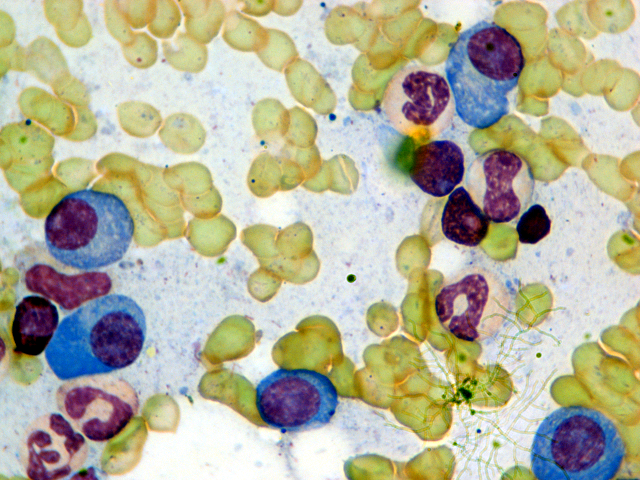
\includegraphics[scale=0.2]{reports/images/cell_00001.png}
        \caption{Original image, 640 x 480}
    \end{subfigure}
    \hfill
    \begin{subfigure}[b]{0.45\textwidth}
        \centering
        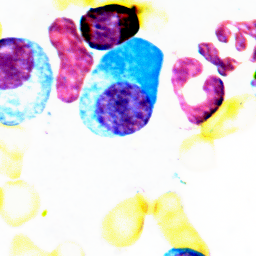
\includegraphics[scale=0.4]{reports/images/transformed_cell_00001.png}
        \caption{Transformed image, 216 x 216}
    \end{subfigure}
    \caption{Comparison of transformed image and original image}
    \label{fig:transformed_images}
\end{figure}

\section{Models}

\subsection{Baseline U-Net}
The U-Net convolutional neural network (CNN) is a widely used model for image segmentation. The competition authors provide a naive U-Net model as a baseline. We utilized this model to gain a better understanding of the data and the appropriate approach for working with it. On the validation data subset, the model achieved an F1 score of 0.418. We used their architecture as an inspiration for ours.

\subsection{Cellpose \& Omnipose}
The Cellpose and Omnipose models are state-of-the-art (SOTA) models for generalized cell segmentation. Using these models was part of our initial project objectives. However, we observed that the competition authors had already experimented with them and found their results to be highly variable. 
\begin{figure}[!h]
    \centering
    \begin{subfigure}[b]{0.45\textwidth}
        \centering
        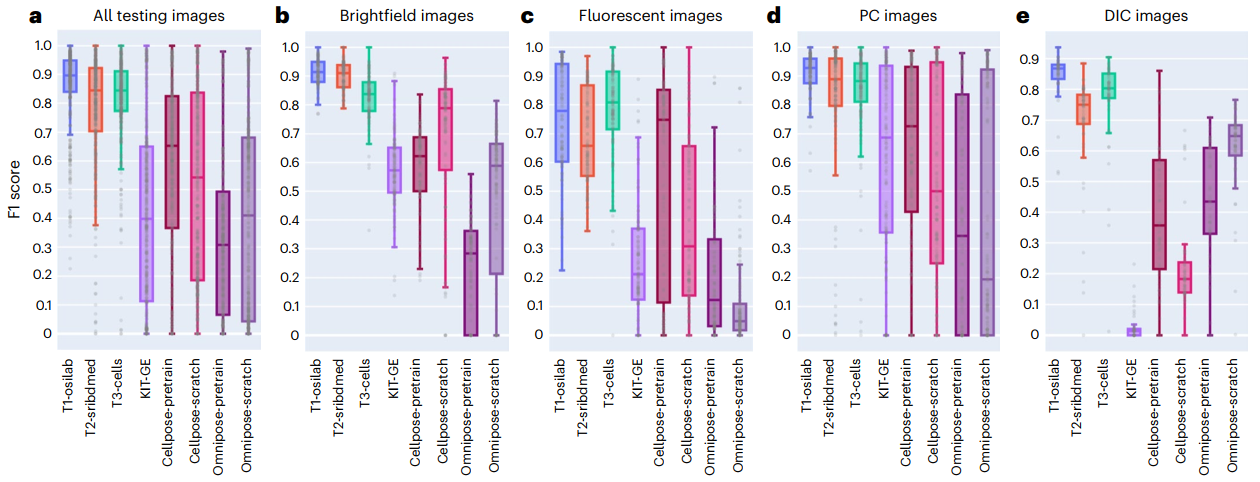
\includegraphics[width=\linewidth]{reports/images/cellpose_competition_stains.png}
        \caption{Dot and box plot of the
F1 scores on the whole testing test}
    \end{subfigure}
    \hfill
    \begin{subfigure}[b]{0.45\textwidth}
        \centering
        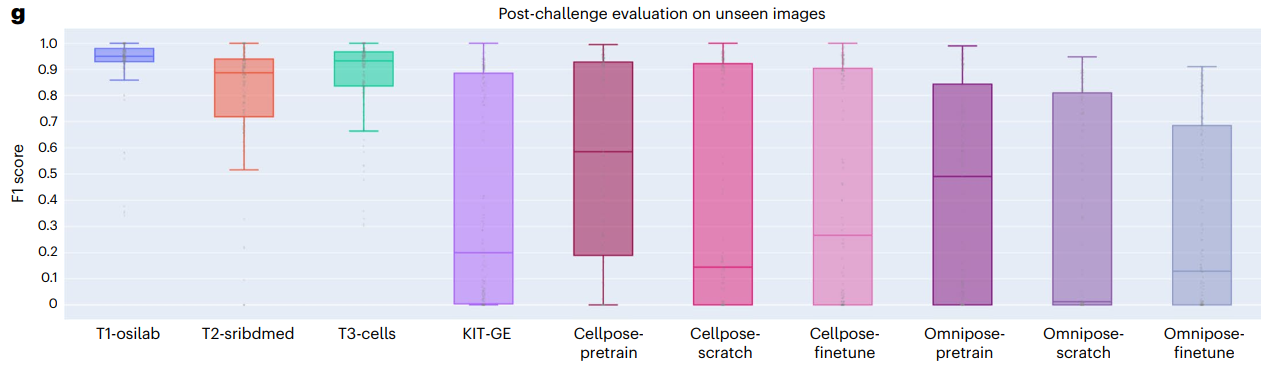
\includegraphics[width=\linewidth]{reports/images/cellpose_competition_test.png}
        \caption{Quantitative comparison on the post-challenge testing set}
    \end{subfigure}
    \caption{Results from the authors of the NeurIPS competition}
    \label{fig:transformed_images}
\end{figure}
\\As a result, we plan to adapt our objectives by using these models in combination with various data augmentation techniques, such as GANs, to assess whether they reduce the variability. This also led us to consider other SOTA segmentation models, such as SAM-2 and YOLO.

\section{Data Augmentation}
A challenge that was flagged by the other competitors was the inefficiency of using unlabeled data. We try a novel way to generate pseudo masks. One solution is to feed the unlabeled images into pretrained segmentation models (SAM-2 and YOLO) to generate the pseudo masks. Another solution is to train a cGAN (Conditional-GAN) that will be trained on the labeled pairs, and use the generator of this trained model to generate masks conditionally to the unlabeled image. 
These solutions are attempts to use the unlabeled for training the segmentation models. Furthermore, we have explored image captioning as a way to augment the images with natural language captions.
\subsection{SAM-2}
Meta's SAM-2 model is another state-of-the-art architecture for universal segmentation. The objective is to exploit an unbalanced dataset (majority of unlabeled images) using SAM2, which generates quality mask.

We began by applying the model directly, and it successfully identified a few cells (see figure below). Although the result is encouraging, it isn't good enough. One approach to explore in the coming weeks is fine-tuning the model using our own data.

\begin{figure}[H]
    \centering
    \begin{subfigure}[b]{0.45\textwidth}
        \centering
        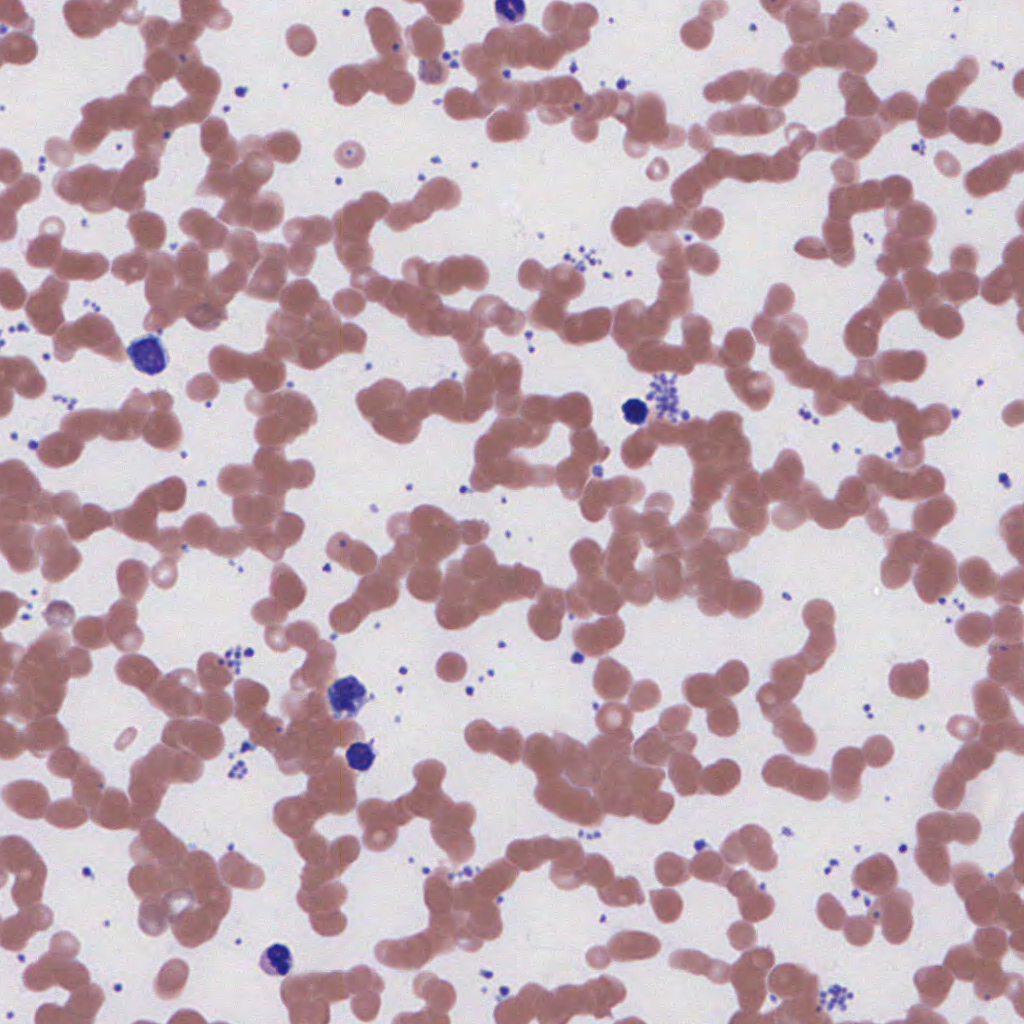
\includegraphics[width=0.45\linewidth]{reports/images/cell_00225.png}
        \caption{Original image}
    \end{subfigure}
    \hfill
    \begin{subfigure}[b]{0.45\textwidth}
        \centering
        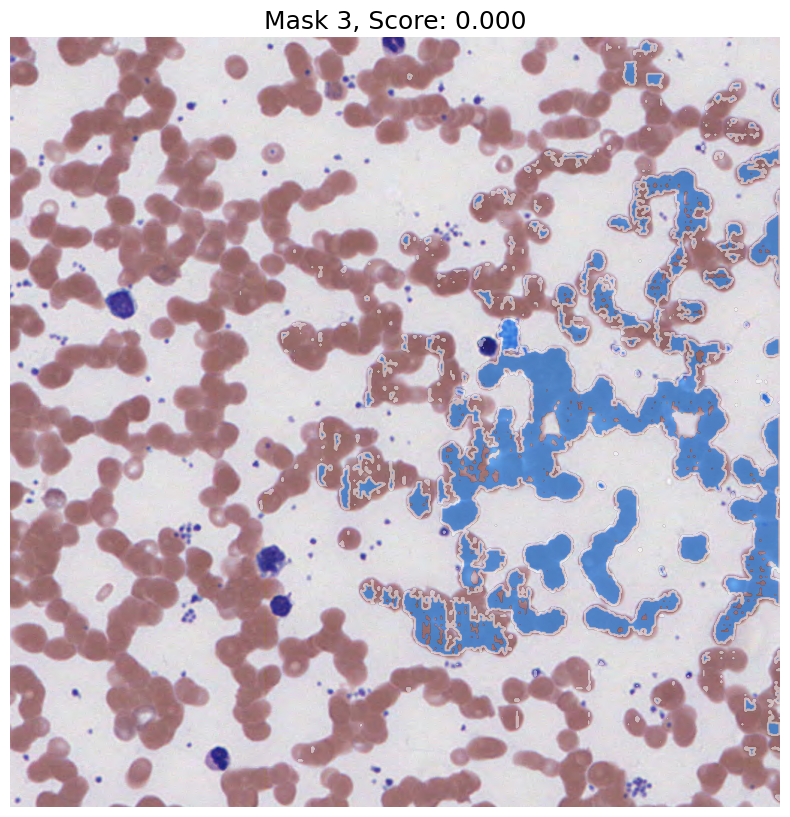
\includegraphics[width=0.45\linewidth]{reports/images/sam2_pretrain_results.png}
        \caption{Masks applied}
    \end{subfigure}
    \caption{SAM-2 pretrained segmentation results}
    \label{fig:transformed_images}
\end{figure}

On the numerous tests carried out, we can notice that the model produces masks comparable to data with a label for certain cell types. However, it tends to over-segment images with purple cells (images containing a very large number of cells overall but with few cells for which we want the masks).

The developed code responds to this challenge with a hybrid approach: post-SAM colorimetric clustering (K-means on HSV space) makes it possible to specifically isolate the masks corresponding to the target (purple) and non-target cells, thus improving the robustness of the model while capitalizing on the available unsupervised data.

\begin{figure}[H]
  \centering
  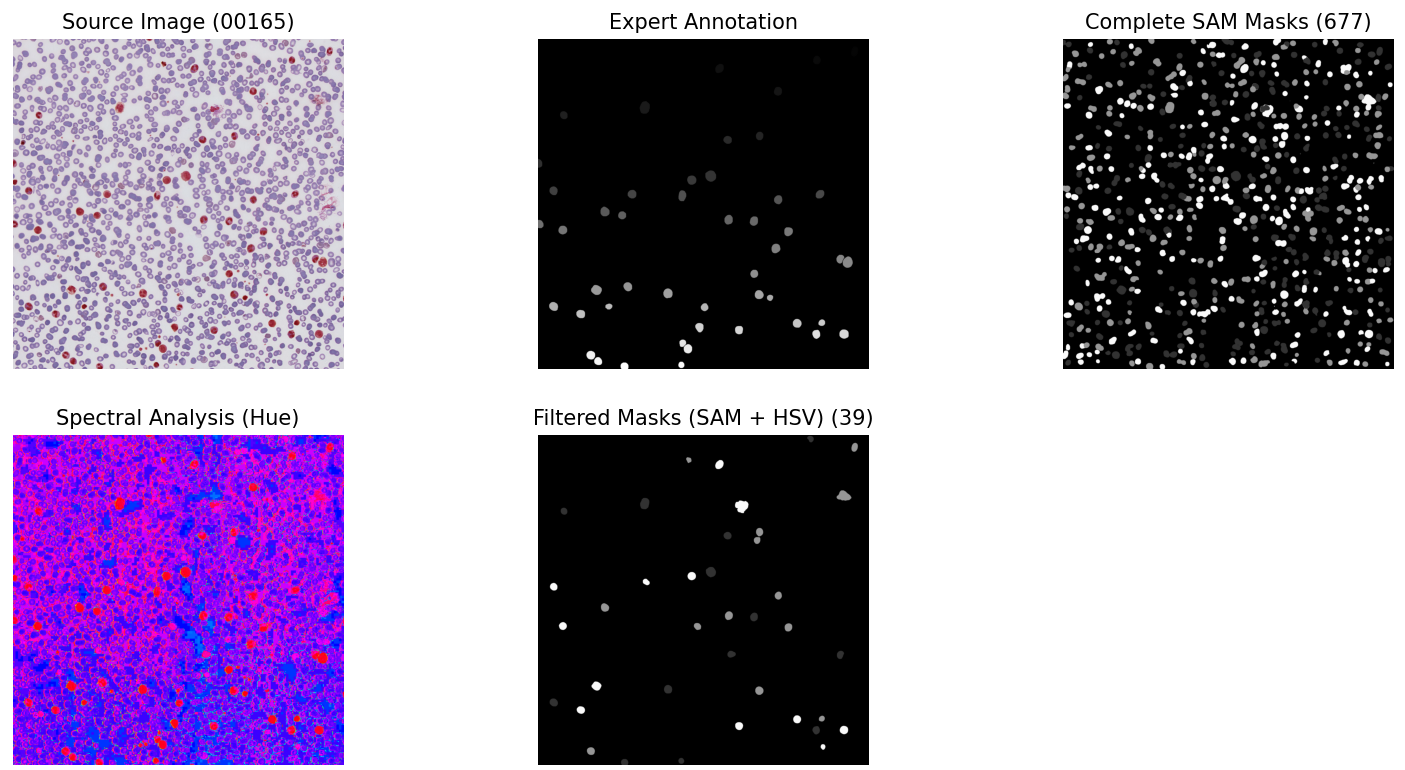
\includegraphics[width=0.8\textwidth]{reports/images/Comparaison_00165.png}
  \caption{SAM-2 model vs SAM-2 + HSV clustering}
  \label{fig:mon_image}
\end{figure}

Overall the SAM-2 model could be used for some cell types, although this will require additional filtering to match expert annotations.


\subsection{YOLO11}
The YOLO11 and YOLO12 models are state-of-the-art (SOTA) architectures designed for universal segmentation. We initially attempted to apply these models directly, but with no success, as none were able to detect a single cell. We then tried fine-tuning the models; however, this required more memory than our available GPU (RTX 3060) could handle, causing the training process to crash. We experimented with various models, including the smallest version (Nano), but unfortunately, all attempts resulted in failure. Further research is needed in the coming weeks to reduce memory requirements or explore alternative solutions, such as leveraging resources from Calcul Québec.

\subsection{Pix2Pix}
Generative Adversarial Networks (GANs) have been widely used for image-to-image translation tasks, and conditional GANs (cGANs) extend this concept by learning a mapping from a source domain \( X \) to a target domain \( Y \) given paired data. In this work, we leverage the Pix2Pix architecture, a cGAN designed for paired image translation, to generate pseudo-masks from raw images.

Instead of employing a traditional segmentation model, we fine-tune Pix2Pix using a corpus of labeled data consisting of \textit{(raw image, segmentation mask)} pairs. The generator \( G \) in the Pix2Pix framework learns to map an input raw image \( x \in X \) to a synthetic segmentation mask \( \hat{y} \in Y \), while the discriminator \( D \) evaluates the realism of the generated mask by distinguishing it from real ground truth segmentation masks. This adversarial setup optimizes the generator to produce segmentation masks that closely resemble human-labeled annotations.


Once the Pix2Pix model is trained, we apply the generator to previously unlabeled raw images to produce synthetic segmentation masks, which we refer to as \textit{pseudo-masks}. These pseudo-masks will then be integrated into a larger training set to improve the performance of a dedicated segmentation model. This approach allows us to expand the labeled dataset without requiring additional manual annotations, leveraging adversarial learning to refine mask generation. That said, we have issues stabilizing the training of this model, a recurring issue with GANs. 

%\subsection{SAM-2}


\subsection{Image captionning}
For image caption generation, we will use transformer-based vision-language models to generate descriptions for both labeled and unlabeled cell images. We will fine-tune a pre-trained \textbf{\textit{BLIP-2}} or \textbf{\textit{OFA}} model, which consists of a Vision Transformer (ViT) as the encoder and a text decoder, such as \textbf{\textit{T5}}, to generate captions. The model will be trained using a cross-entropy loss function and evaluated using \textbf{\textit{BLEU}}, \textbf{\textit{CIDEr}}, and \textbf{\textit{METEOR}} scores. To improve caption quality, we will apply a filtering process using cosine similarity between generated captions and existing ones, ensuring relevance and coherence. Additionally, we will augment captions by using \textbf{\textit{T5}} for paraphrasing, \textbf{\textit{WordNet}} for synonym replacement, and back-translation techniques to enhance diversity. The key libraries include transformers for model fine-tuning, sentence-transformers for similarity scoring, and \textbf{\textit{deep-translator}} for back-translation. This approach will enrich our dataset with meaningful textual descriptions, potentially improving the performance of the cell segmentation model.

\section{Next steps}
Over the next two weeks, the team will focus on finalizing the data augmentation process. Kamen will work on stabilizing Pix2Pix training and generating pseudo-masks to be used for training the segmentation models. Johann will continue experimenting with pretrained segmentation models, validating their effectiveness both quantitatively and qualitatively. Samir will refine caption augmentation by cross-validating different models and prompts, while also enhancing preprocessing by developing a cropping script to extract more labeled samples from large images. Simon and Guillaume, who are focused on segmentation, will continue exploring new versions of the leading cell segmentation models, such as Cellpose 3.0 and Omnipose, while also actively contributing to finalizing the data augmentation step. By the end of these two weeks, we expect to have fully augmented datasets and models ready for training. The following phase will involve running trials with different augmentation strategies and model architectures, conducted in parallel with paper writing, presentation preparation, and demo development.
\end{document}